% !TEX encoding = UTF-8
% !TEX TS-program = pdflatex
% !TEX root = ../../tesi.tex

\section{Studio preliminare}
Durante la fase di studio preliminare ho dovuto apprendere tutte le nozioni teoriche che stanno alla base del funzionamento della \textbf{tecnologia \textit{blockchain}} e, in seguito, alla base delle \textit{blockchain} \textbf{Ethereum} e \textbf{Hotmoka}, con i relativi linguaggi per la scrittura di \textit{smart contract}.

\subsection{Cos'è la blockchain}
La \textit{blockchain} è una nuova tipologia di registro distribuito strutturato come una catena di blocchi contenenti le transazioni. Fa parte, perciò, della più ampia famiglia delle tecnologie di \textbf{\textit{Distributed Ledger}}, ossia sistemi che si basano su un registro distribuito che può essere letto e modificato da più nodi di una rete. 

In più, un'altra caratteristica molto importante della \textit{blockchain} è il fatto di essere \textit{permissionless}, ovvero chiunque può connettersi alla rete e far parte del complesso sistema che la regola. Questo rende tutto molto più complesso dato che, reti come questa, hanno bisogno di regole del consenso molto più forti rispetto a reti \textit{permissioned}, per assicurare la validità e il funzionamento corretto del sistema. \\

\noindent Le caratteristiche della tecnologia \textit{blockchain}, riassumendo, sono le seguenti:
\begin{itemize}
  \item \textbf{Decentralizzazione}: le informazioni vengono registrate distribuendole tra più nodi per garantire sicurezza informatica e resilienza dei sistemi;
  \item \textbf{Tracciabilità dei trasferimenti}: ciascun elemento sul registro è tracciabile in ogni sua parte e se ne può risalire all’esatta provenienza;
  \item \textbf{Disintermediazione}: le piattaforme consentono di gestire le transazioni senza intermediari, ossia senza la presenza di enti centrali fidati;
  \item \textbf{Trasparenza e verificabilità}: il contenuto del registro è trasparente e visibile a tutti ed è facilmente consultabile e verificabile;
  \item \textbf{Immutabilità del registro}: una volta scritti sul registro, i dati non possono essere modificati senza il consenso della rete;
  \item \textbf{Programmabilità dei trasferimenti}: possibilità di programmare determinate azioni che vengono effettuate al verificarsi di certe condizioni, anche se nella \textit{blockchain} originale di BitCoin è permesso.
\end{itemize}

Per comprendere al meglio come funzionano tutti questi meccanismi, introduciamo ed approfondiamo la prima \textit{blockchain} che sia mai stata creata, ovvero BitCoin. \\

\textbf{BitCoin} è nata alla fine del 2009, quando Satoshi Nakamoto, una persona o un gruppo di persone la cui identità è tutt'ora ignota, pubblica un \textit{white paper} spiegando la sua idea di moneta virtuale crittografica \textit{peer-to-peer} senza intermediari. Di seguito potremo analizzare più approfonditamente come funziona questa tecnologia.

\paragraph{Il wallet}
Il concetto di \textit{wallet}, o portafoglio in italiano, è importantissimo e permette a chiunque di interagire con la \textit{blockchain}. Consistono in applicativi \textit{software} che permettono la compravendita della criptovaluta BitCoin. Il \textit{wallet} ha lo stesso compito del codice IBAN di un conto corrente.

Ogni \textit{wallet} ha un indirizzo, il quale viene creato attraverso un processo di manipolazione di una chiava privata che si ottiene generando un numero casuale tra 0 e 2\textsuperscript{256}-1, attraverso un generatore di numeri casuali uniformemente distribuito, dove vengono utilizzati algoritmi che generano numeri con la stessa probabilità. Questa chiave privata viene creata localmente ed è importantissima in quanto tutte le transazioni vengono firmate digitalmente con essa e permette l'accesso al proprio \textit{wallet}. Se viene rubata non si può fare altro, se non rassegnarsi d'aver perso tutti i propri BitCoin.

Dalla chiave privata attraverso l'applicazione della funzione di ECDSA-512, viene ottenuta la chiave pubblica e, in seguito, dalla chiave pubblica si ottiene l'indirizzo del \textit{wallet} applicando la funziona di hash RipeMD160 e convertendo il risultato in \textit{base58} per una migliore comprensione di quest'ultimo. Inoltre dall'indirizzo del \textit{wallet} sono state rimosse tutte le lettere o numeri ambigui come lo sono zero e la lettera O.

\begin{figure}[h!]
  \centering
  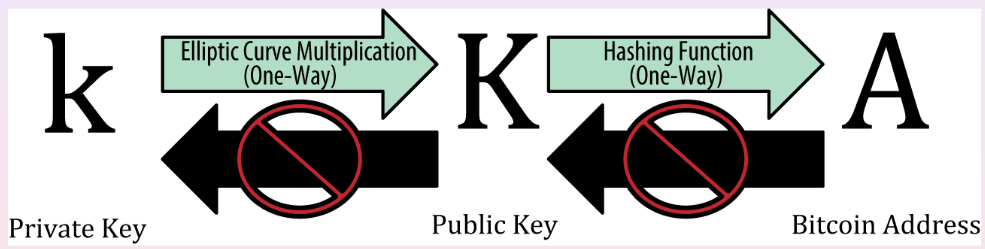
\includegraphics[width=\textwidth]{capitolo3/studio-preliminare/bitcoin-keys.png}
  \caption{Flusso di generazione del \textit{wallet} in BitCoin}
  \textbf{Fonte}: \href{https://github.com/spoto/blockchain-course}{Corso dell'università di Verona sulla tecnologia \textit{Blockchain}} 
\end{figure}

Data l'attenzione che bisogna dedicare alla sicurezza della chiave privata sono nati molte tecniche per facilitarne la memorizzazione. Una di queste tecnologie così importanti sono i \textbf{Deterministic Wallet}, ovvero non bisognerà ricordarsi la chiave privata associata ad ogni \textit{wallet} che una persona ha, ma ci sarà una \textit{Master Private Key} da cui si potranno derivare in maniera deterministica tutte le altre chiavi private, dalle quale si otterranno gli indirizzi dei \textit{wallet}. 

Un'altra soluzione che sta sempre di più prendendo piede è l'utilizzo delle 12 parole. La chiave privata, in questo caso, viene associata a 12 parole che vengono pescate da un vocabolario di circa 2048 parole. In seguito verrà anche associata ad una password personale, la combinazione della password e delle dodici parole permette di ricondursi alla chiave privata originale. Questo permette una maggiore facilità di memorizzazione, non dovendosi portare dietro la chiave privata scritta da qualche parte.   

\paragraph{Come si svolge una transazione}
Per comprendere al meglio come si svolge una transazione in BitCoin, dobbiamo prima comprendere come vengono gestiti i bilanci dei vari \textit{wallet}. BitCoin stravolge il paradigma applicato ai sistemi bancari attuali dove si ha una determinata somma di denaro e a questa viene sottratta o aggiunta una somma di denaro in base alla situazione. Il modello utilizzato da BitCoin, invece, si chiama \textit{UTXO} (\textit{Unspent Transaction Output}) dove un \textit{wallet} possiede tutte le transazioni assegnate a lui. Per calcolare il bilancio, perciò, bisognerà analizzare tutte le transazioni non spese che sono assegnate a quello specifico \textit{wallet}.

\begin{figure}[h!]
  \centering
  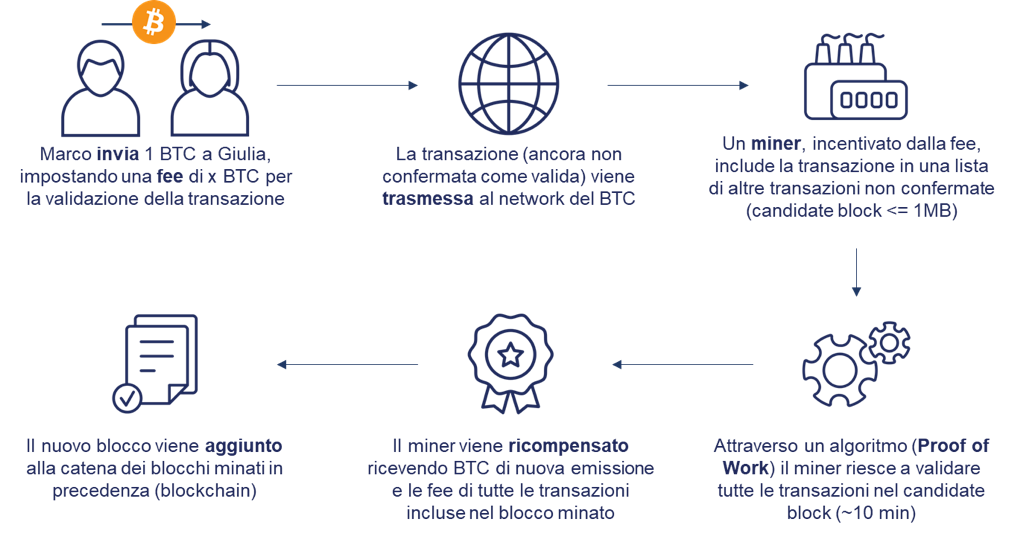
\includegraphics[width=\textwidth]{capitolo3/studio-preliminare/bitcoin-transaction.png}
  \caption{Esecuzione di una transazione in BitCoin}
  \textbf{Fonte}: \href{https://www.focusmgmt.it/knowledge/innovazione-nella-blockchain-il-lightning-network/}{https://www.focusmgmt.it/knowledge/innovazione-nella-blockchain-il-lightning-network/}
\end{figure}

Quando si verifica una transazione, cioè lo scambio di BitCoin da un \textit{wallet} ad un altro, questa viene diffusa a tutti i \textit{peer} della rete per essere elaborata. A questo punto entrano in gioco i \textit{\textbf{miner}}, ovvero \textit{peer} che hanno il compito di validare le transazioni ed inserirle dentro i blocchi della \textit{blokchain}. Ogni \textit{miner} fa questo per ottenere la commissione che viene pagata dal mittente del pagamento e un tasso di inflazione che immette moneta nella rete. come verrà spiegato in seguito. 

Appena un \textit{miner} riceve una transazione la colloca dentro la \textit{mining pool}, ovvero un grande contenitore dove vengono posizionate tutte le transazioni che ha ricevuto e che deve elaborare. Di solito, per la complessità di questo processo, il \textit{miner} seleziona solo quelle con la commissione più alta in modo da avere il ricavo maggiore.

In seguito avviene a creazione del blocco con le transazioni scelte e, cosa più importante, avviene anche il processo di \textit{proof of work}. Il \textit{proof of work} consiste in un processo che obbliga il minatore ad allegare al blocco una prova di un lavoro compito. Questo lavoro consiste nel trovare un numero, chiamato \textit{\textbf{nonce}}, che inserito dentro il \textit{header} del blocco faccia si che l'hash del singolo \textit{header} sia minore di un valore intrinseco della rete, variabile in determinato intervallo, chiamato \textit{difficulty}. È lavoro molto pesante e serve a non incoraggiare la creazione di blocchi falsi e malevoli. Attualmente, per come è stata impostata la difficulty della rete, un minatore ci mette 10 minuti a generare un blocco valido.

Quando avrà ottenuto il blocco valido, lo condividerà a tutta la rete per informare tutti quali transazioni ha validato e condividere lo stato della sua \textit{blockchain} interna. Gli altri \textit{peer} valideranno il blocco controllando che tutti i campi siano corretti e lo accetteranno in tal caso. A questo punto il miner potrà prendere la sua ricompensa composta dalle commissioni delle transazioni che ha validato. Dato che la validazione delle transazioni è un processo mutualmente esclusivo, ma tutti possono concorrere per la loro validazione, quando viene informata la rete dell'aggiunta di un nuovo blocco con annessa validazione delle transazioni al suo interno, tutti gli altri \textit{peer} controllano le transazioni che sono state appena validate e, nel caso in cui ce ne siano di già validate che sta validando anche lui, dovrà scartare il blocco e ricominciarlo da capo, non percependo alcuna ricompensa.

\paragraph{Composizione di un blocco in BitCoin}
\begin{figure}[h!]
  \centering
  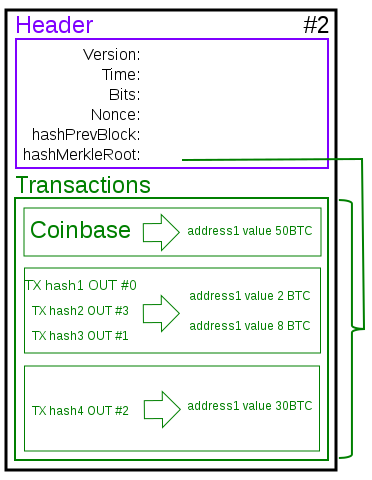
\includegraphics[width=0.4\textwidth]{capitolo3/studio-preliminare/bitcoin-block-structure.png}
  \caption{Composizione di un blocco in BitCoin}
\end{figure}

Un blocco in BitCoin è composto nel seguente modo:
\begin{itemize}
  \item \textbf{\textit{Header} del blocco}:
  \begin{itemize}
    \item \textbf{Hash del blocco precedente};
    \item \textbf{\textit{Timestamp}}: \textit{timestamp} di creazione del blocco;
    \item \textbf{\textit{Difficulty}}: valore intrinseco della rete e variabile in un intervallo che serve alla \textit{proof of work};
    \item \textbf{\textit{Nonce}}: prova di lavoro che si porta dietro il blocco;
    \item \textbf{\textit{Merkle root}}: hash della radice del \textit{Merkle Tree} delle transazioni.
  \end{itemize}
  
  \item \textbf{Transazioni}: dove sono presenti tutte le transazioni validate nel blocco.
\end{itemize}

Un \textit{Merkle Tree} è una struttura dati che la tecnologia \textit{blockchain} utilizza per la verifica della validità di una transazione con modalità \textit{Zero knowledge proof}.

\begin{figure}[h!]
  \centering
  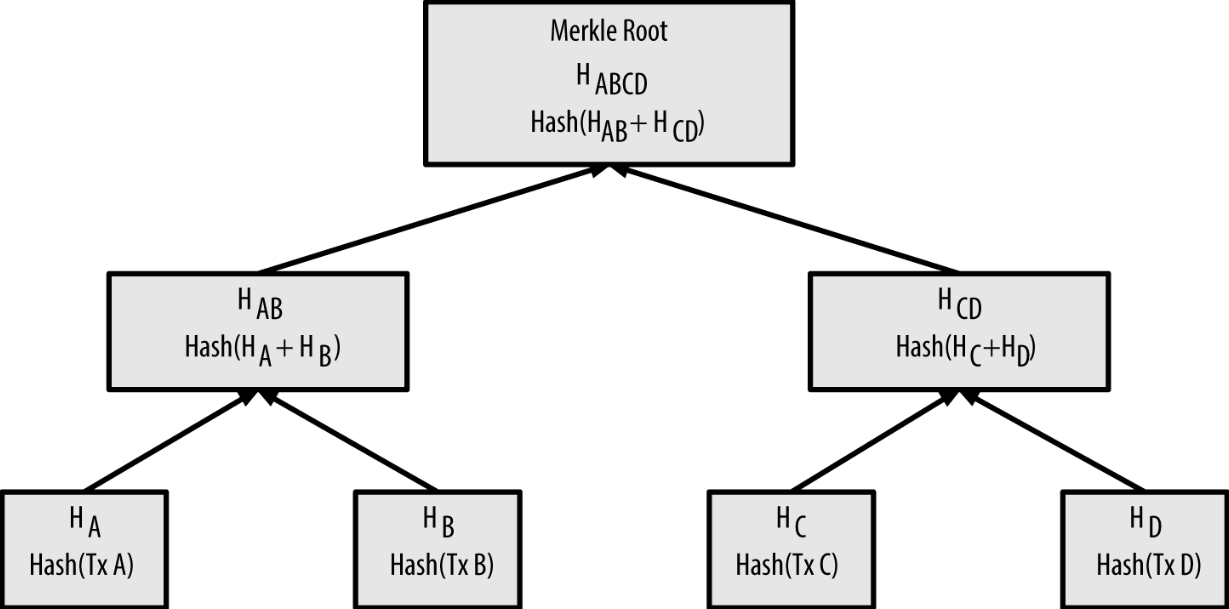
\includegraphics[width=\textwidth]{capitolo3/studio-preliminare/bitcoin-merkle-tree.png}
  \caption{Esempio di Merkle Tree}
\end{figure}

Consiste in un albero binario sempre bilanciato nel quale alle foglie sono presenti tutte le transazioni interne al blocco. Ogni nodo non foglia avrà come valore l'hash tra l'hash dei suoi figli. In questo modo un qualsiasi \textit{peer} può verificare che una transazione sia valida e all'interno di un determinato blocco chiedendo semplicemente ad un \textit{full node} (nodo con tutta la \textit{blockchain} memorizzata) di verificarla. Lui gli invierà le transazioni che permetteranno di risalire al \textit{Merkle Root} del nodo a partire dalla transazione che vuole verificare, semplicemente eseguendo l'hash tra i seguenti blocchi.

\clearpage
\begin{figure}[h!]
  \centering
  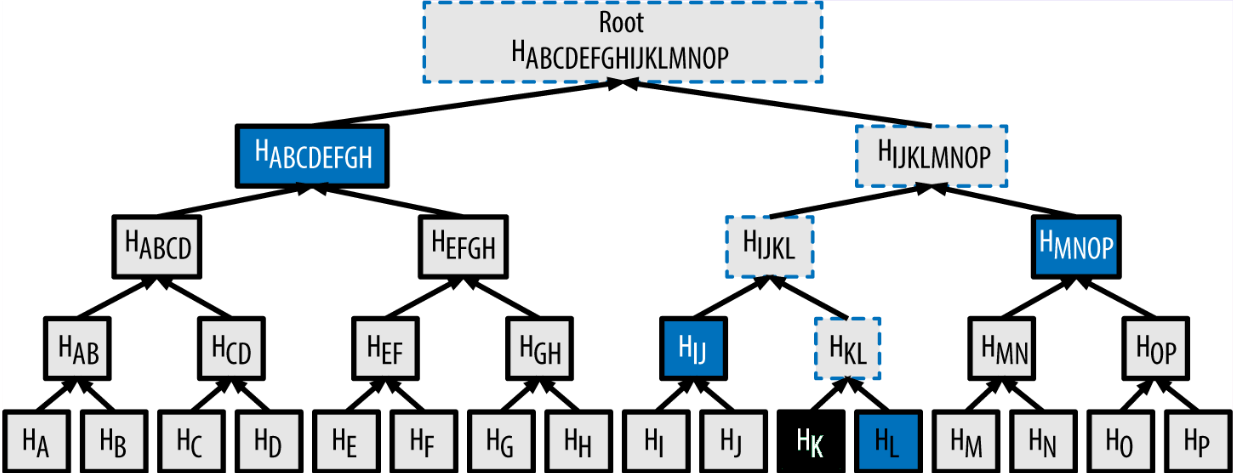
\includegraphics[width=\textwidth]{capitolo3/studio-preliminare/bitcoin-merkle-tree-verify.png}
  \caption{Esempio di verifica di una transazione in un Merkle Tree}
  \label{fig:merkle-tree-verify}
\end{figure}

Ad esempio, come si può vedere in figura \ref{fig:merkle-tree-verify}, per verificare che la transazione H\textsubscript{k} sia effettivamente in un nodo, allora si chiederà ad un \textit{full node} di mandargli tutte le transazioni colorate in colore blu. A questo punto il \textit{peer} richiedente potrà ottenere tutti i nodi tratteggiati di blu fino ad arrivare alla radice. A questo punto basterà confrontare l'hash della radice ottenuta e quella presente nel blocco. Se corrispondono significa che è presente in quel blocco. 

\paragraph{Le diramazioni in BitCoin}
Essendo la \textit{blockchain} un sistema distribuito, deve fare anche i conti con il problema dell'inconsistenza dei dati e delle possibili diramazioni della storia delle transazioni che si creano ogni secondo.

Non è rara la situazione in cui un nodo sia il precedente di due nodi. BitCoin risolve questo problema mantenendo come storia principale quella con più nodi e non accettando più aggiunte di un blocco che ha come nodo precedente un nodo di una diramazione non più valida.

\paragraph{Sicurezza nella Blockchain}
Come ultima accenniamo la sicurezza della \textit{Blockchain}, visto che è doveroso parlarne.

L'attacco più famoso e pericolo che si possa attuare in BitCoin, o in \textit{blockchain} che utilizzano come algoritmo \textit{proof-of-work}, consiste nell'attacco del 51\%.

Questo attacco avviene quando una persona, o un gruppo di persone, detiene il potere computazionale del 51\%. Salta così il concetto di rete decentralizzata, infatti avendo il controllo della maggioranza della potenza di calcolo si potrà decidere aggiungere nuovi blocchi, manipolare le operazioni bidirezionali e rifiutarsi di confermare le nuove transazioni. 

Attraverso questo attacco è possibile eseguire anche il \textit{double spending}, ovvero illudere il sistema di non aver speso una transazione e riutilizzarla effettuare un altro acquisto.

C'è da dire che non si è mai verificato un caso di questo attacco in un \textit{blockchain} grande come lo è BitCoin o lo può essere Ethereum, visto che sono troppo distribuite nel mondo e risulta quasi impossibile riuscire ad avere il 51\% della potenza di calcolo totale.  

%%%%%%%%%%%%%%%%%%%%%%%%%%%%%%%%%%%%%%%%%%%%%%%%%%%%%%%%%%%%%%%%%%%%%%%%%%%%%%%%%%% 

\subsection{La blockchain Ethereum}
La \textit{blockchain} Ethereum è nata nel 2014 da un'idea di Vitalik Buterin e Gavin Wood. Quello che hanno voluto creare è una \textit{blockchain} programmabile attraverso programmi chiamati \textit{smart contract} che possono essere installati all'interno di blocchi della \textit{blockchain}. \\

Sotto molti aspetti non si differenzia di molto da BitCoin per quanto riguarda il funzionamento del consenso, la composizione dei blocchi e la creazione del \textit{wallet}, tranne per qualche funzione crittografica utilizzata. La grande differenza rispetto a BitCoin è che viene introdotto il concetto di stato di un blocco. Infatti se prima ogni transazione in BitCoin corrispondeva alla generazione di una \textit{UTX}, ora viene generalizzato questo concetto corrispondendo ad un cambiamento dello stato di un blocco.

\paragraph{Il concetto di smart contract}
Uno \textit{smart contract} è un programma installabile all'interno di una \textit{blockchain} con il quale ci permette di scambiare valuta o modificare lo stato di entità presenti in modo trasparente senza conflitti evitando servizi di terze parti. \\

Le caratteristiche di uno \textit{smart contract} sono:
\begin{itemize}
  \item \textbf{Immutabilità}: il codice di uno \textit{smart contract} caricato in \textit{blockchain} non può essere modificato, ma bisognerà caricarne uno nuovo;
  \item \textbf{Irrevocabilità}: non può essere cancellato;
  \item \textbf{Deterministico}: non possono essere utilizzati metodi non deterministici, come la generazione di numeri casuali, perché ad ogni operazione deve corrispondere sempre e solo un rispettivo output e queste devono ripetibili in caso di riallineamento della stato;
  \item \textbf{Terminabile}: anche se i linguaggi di programmazione con cui si possono scrivere \textit{smart contract} sono turing completi, sono stati applicati dei sistemi per far si che termini sempre. Questo perchè non si possono fermare dei \textit{peer} della rete per l'esecuzione di uno \textit{smart contract} che non termina;
  \item \textbf{Isolato}: tutti i cambiamenti di stato devono essere eseguiti in un ambiente indipendentemente dal \textit{peer} della rete. Per questo esiste la \textit{EVM} (\textit{Ethereum Virtual Machine}).
\end{itemize}

Con uno \textit{smart contract} si può:
\begin{itemize}
  \item far eseguire computazioni ai \textit{peer} della rete distribuita della \textit{blockchain};
  \item mantenere la persistenza di dati;
  \item trasferire soldi (ether) da un \textit{EOA} a un qualsiasi altro \textit{EOA}.
\end{itemize}

Per rendere sempre terminabile uno \textit{smart contract}, Ethereum ha introdotto il concetto di \textit{Gas limit} e \textit{Gas price}.

Il \textbf{Gas limit} è la massima quantità di \textit{Gas} che si è disposti a spendere. Il \textit{Gas price}, invece, è il prezzo al quale si è disposti a spendere il \textit{Gas} e viene calcolato in Gwei (la più piccola unità della moneta Ether). Insieme compongono quanto si è disposti a spendere per l'esecuzione di un'operazione, ovvero \textit{Gas limit} * \textit{Gas price}. Infatti istruzione che viene eseguita in uno \textit{smart contract} ha un costo in Gwei più o meno alto in base a quello che fa. Quando le operazioni eseguite in uno \textit{smart contract} superano, in prezzo, quanto si è disposti a spendere allora lo \textit{smart contract} terminerà l'esecuzione. Questo ha reso impossibile, ad esempio, la realizzazione di cicli infiniti.\\

Il linguaggio più utilizzato e ufficiale per la scrittura di \textit{smart contract} è Solidity. Essendo finalizzato solo alla scrittura di \textit{smart contract} è un linguaggio che presenta molti costrutti che ne facilitano lo sviluppo.

\begin{figure}[h!]
  \centering
  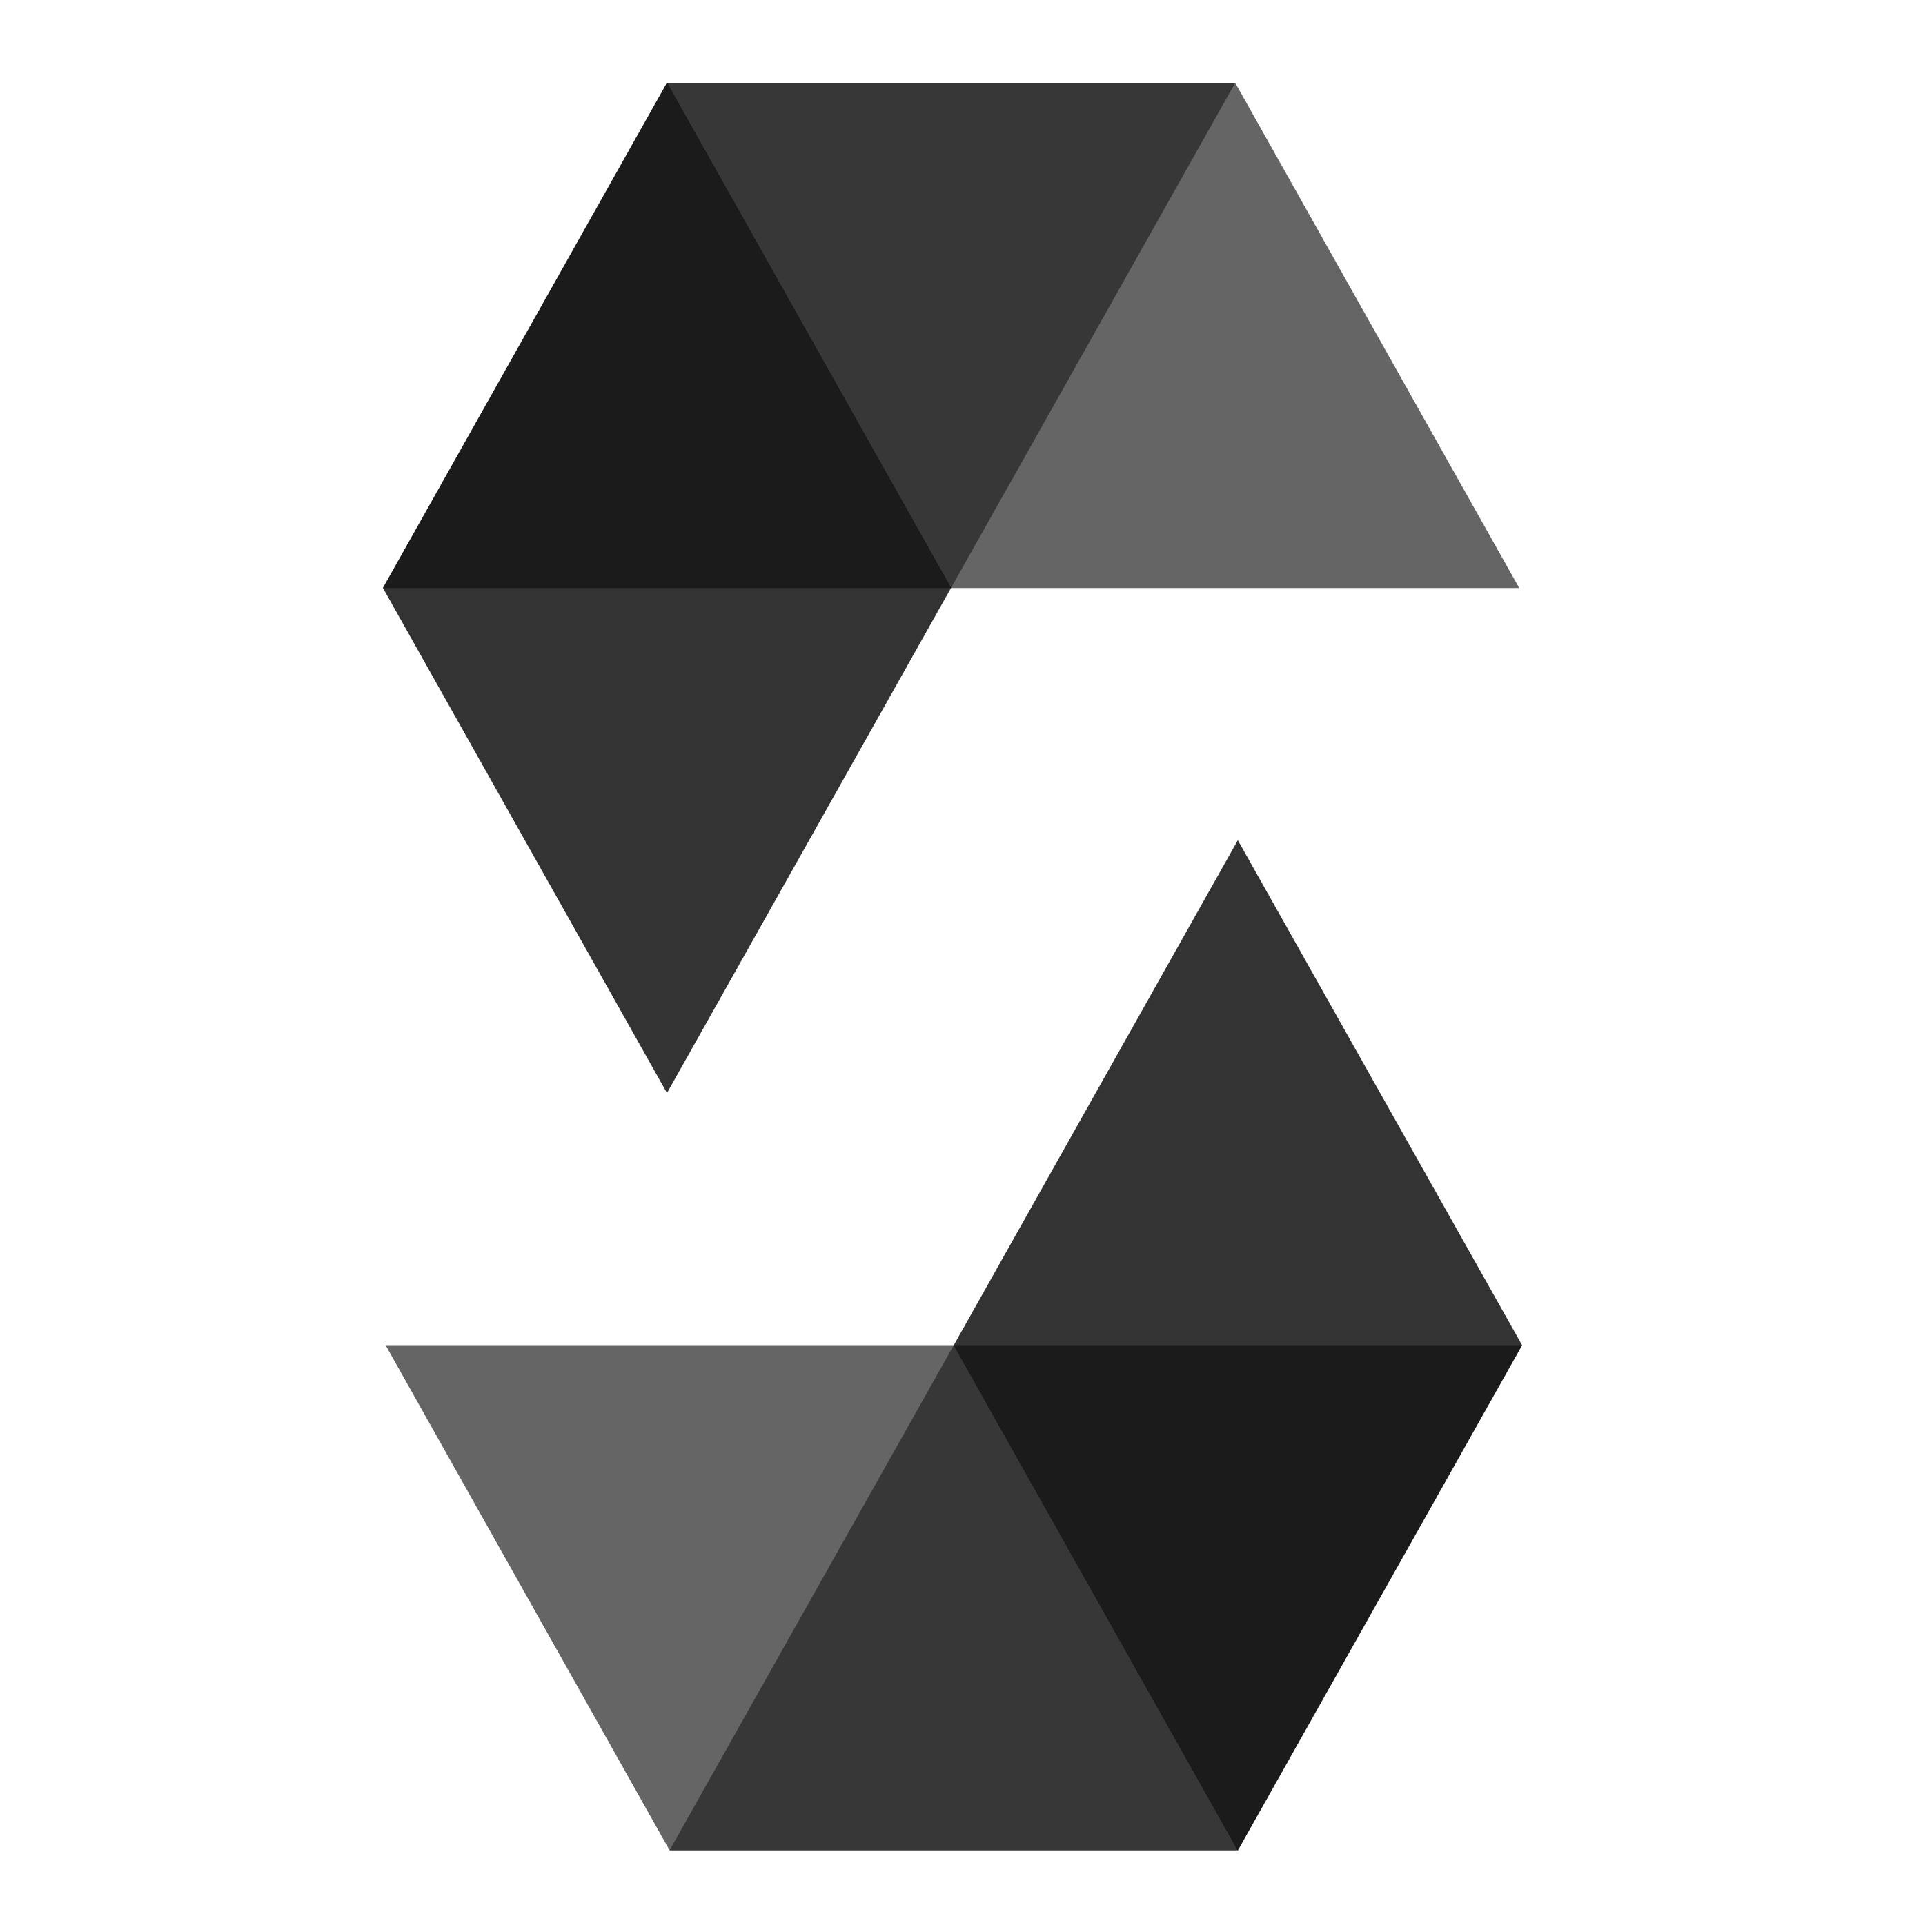
\includegraphics[width=0.3\textwidth]{capitolo3/solidity-logo.png}
  \caption{Logo di Soldity}
\end{figure}

Alcuni costrutti degni di nota sono:
\begin{itemize}
  \item non esiste il \textit{null} e tutte le variabili, se non assegnate in fase di creazione, avranno un valore di \textit{default} in base al loro tipo;
  \item le funzioni che non modificano lo stato dello \textit{smart contract} possono essere classificate come \textbf{\textit{view}} e non verrà speso del \textit{Gas} per eseguirle;
  \item la presenza di modificatori, ovvero funzioni che eseguono del codice prima, o dopo, una funzione. Vengono per lo più utilizzati per la dichiarazione di condizioni d'esecuzione di una funzione, cioè se non rispetta una regola non può essere eseguita. Riducono di molto le ripetizioni di codice e permettono l'implementazione di vari \textit{design pattern}; 
  \item possono essere dichiarati e lanciati eventi che segnalano al mondo esterno allo \textit{smart contract}, l'avvenimento di qualcosa;
  \item la presenza della funzione \textit{built-in} chiamata \textit{require}, la quale permette di far fallire l'esecuzione dello \textit{smart contract} se non viene rispettata una determinata condizione.
\end{itemize}

\paragraph{Tipi di transazioni}
Grazie all'introduzione degli \textit{smart contract} vengono ampliate le tipologie di transazione che si possono eseguire. Viene anche introdotto il concetto di \textit{EOA} (\textit{Externally Owned Accounts}), il quale rappresenta qualsiasi elemento che nella \textit{blockchain} Ethereum può ricevere o inviare soldi (anche uno \textit{smart contract}). \\

\noindent I tipi di transazioni sono i seguenti:
\begin{itemize}
  \item \textbf{Scambio di moneta}: questo è l'unico tipo di transazione dove il destinatario può essere anche un \textit{wallet}. Nel caso in cui sia un \textit{wallet} allora verranno inviati i soldi. Nel caso in cui, invece, l'\textit{EOA} sia un contratto, verrà incrementato il bilancio interno allo \textit{smart contract} invocando un metodo di tipo \textit{payable} oppure utilizzando quello di \textit{fallback};
  
  \begin{figure}[h!]
    \centering
    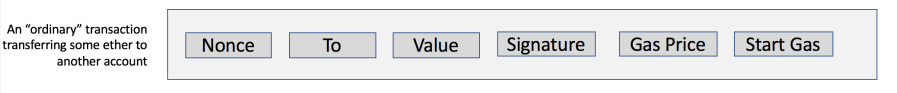
\includegraphics[width=\textwidth]{capitolo3/studio-preliminare/ethereum-transaction-send-money.png}
    \caption{Transazione di scambio di moneta in Ethereum}
  \end{figure}

  \item \textbf{Creazione di un contratto}: consiste in una transazione dove viene eseguita l'installazione di un contratto all'interno di un blocco. In questo caso il campo \textit{to} verrà impostato con valore 0. In seguito all'installazione verrà ritornato l'indirizzo del blocco dove è stato installato lo \textit{smart contract};
  
  \begin{figure}[h!]
    \centering
    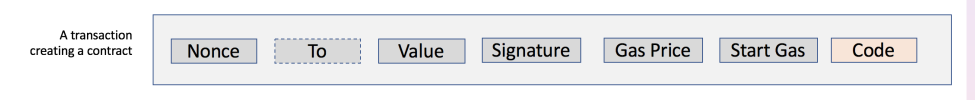
\includegraphics[width=\textwidth]{capitolo3/studio-preliminare/ethereum-transaction-create-contract.png}
    \caption{Transazione di creazione di un nuovo contratto in Ethereum}
  \end{figure}
  
  \item \textbf{Invocazione di un contratto}: consiste in una transazione dove viene invocato un metodo presente in uno \textit{smart contract} precedentemente installato. In questo caso il campo \textit{to} corrisponderà all'indirizzo dello \textit{smart contract} da invocare e il campo \textit{data} il metodo da invocare.
  
  \begin{figure}[h!]
    \centering
    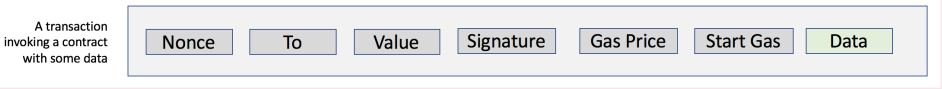
\includegraphics[width=\textwidth]{capitolo3/studio-preliminare/ethereum-transaction-invoke-contract.png}
    \caption{Transazione di invocazione di un contratto in Ethereum}
  \end{figure}
\end{itemize}

\paragraph{Lo stato di Ethereum}
Lo stato in Ethereum è molto complesso e si affida ad una struttura dati chiamata \textit{\textbf{Merkle PATRICIA tries}}, in quanto delle semplice mappe chiave valore non possono permettere il \textit{checkout} di operazioni. Infatti la principale necessità dello stato di Ethereum è la possibilità di eseguire l'operazione di \textit{checkout} tornando indietro nello stato stesso di Ethereum ed eseguire di nuovo tutte le operazioni. Questo perchè, in caso di diramazioni dello stato, qui non è possibile ignorarle e prendere la storia più lunga, come fa BitCoin, ma trattandosi di operazioni bisogna allineare lo stato e rieseguirle.

Il \textit{PATRICIA Trie} è un albero che permette di conversare una serie di dati di tipo chiave valore e poi di recuperarli in modo semplice ed efficiente. La chiave indica il percorso da seguire per giungere alla foglia che contiene il valore corrispondente. Nel caso di Ethereum, il \textit{PATRICIA Trie} viene modificato con concetti visti nel \textit{Merkle Tree}, come ad esempio il fatto che il puntatore ad un nodo è l'hash crittografico del nodo stesso.

%%%%%%%%%%%%%%%%%%%%%%%%%%%%%%%%%%%%%%%%%%%%%%%%%%%%%%%%%%%%%%%%%%%%%%%%%%%%%%%%%%%

\subsection{La blockchain Hotmoka}
Hotmoka è un \textit{framework} per la programmazione di una rete \textit{peer-to-peer}, attraverso un sottoinsieme di Java chiamato Takamaka. I nodi possono appartenere a una \textit{blockchain} o possono essere dispositivi \textit{IOT} (\textit{Internet Of Things}). È sviluppata e mantenuta dall'Università di Verona.

\paragraph{Cos'è Tendermint e il suo utilizzo in Hotmoka}
Tendermint è un framework per la scrittura di \textit{blockchain}. Infatti, come si può vedere in figura \ref{fig:tendermint-structure} il \textit{core} di Tendermint ha solo il compito di gestire i blocchi della \textit{blockchain} e comunicare con gli altri \textit{peer} della essa.

Ciò che viene demandato al programmatore è lo sviluppo del \textit{application layer}, ovvero la definizione di tutto quello che viene memorizzato nella \textit{blockchain}. Per comunicare con il Tendermint core e rendere tutto il più possibile indipendentemente dall'implementazione, l'\textit{application layer} definisce solamente una serie di funzioni che verranno richiamate durante il salvataggio di un blocco da parte del \textit{core} attraverso \textit{sockets}.

\begin{figure}[h!]
  \centering
  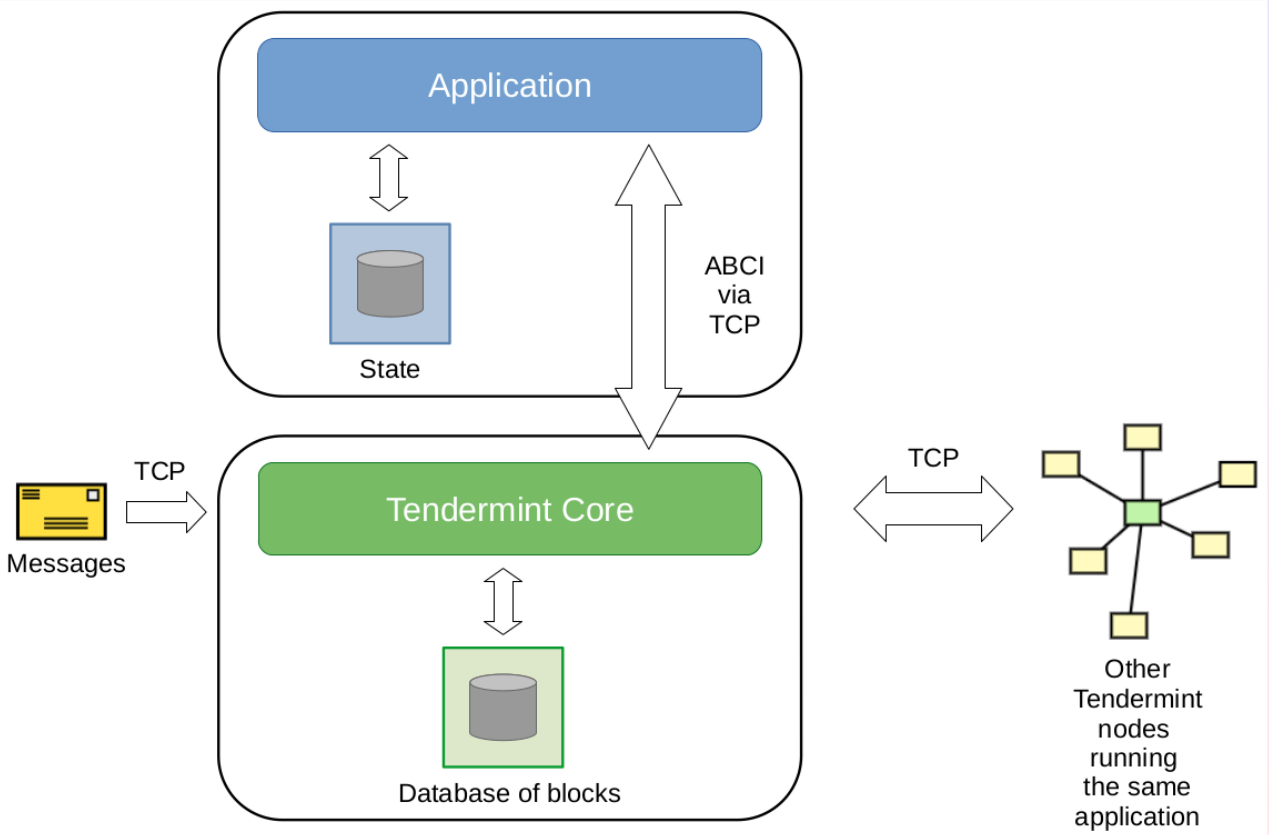
\includegraphics[width=0.8\textwidth]{capitolo3/studio-preliminare/tendermint-structure.png}
  \caption{Struttura di Tendermint}
  \label{fig:tendermint-structure}
\end{figure}

\noindent Le funzioni da implementare sono le seguenti:
\begin{itemize}
  \item \textbf{\textit{checkTX}}: ha il compito di filtro per le transazioni in ingresso, controllando la loro forma sintatticamente corretta;
  \item \textbf{\textit{beginBlock}}: chiamata all'inizio del blocco, riceve informazioni circa l'insieme dei validatori e quali hanno firmato il blocco precedente;
  \item \textbf{\textit{deliverTX}}: viene chiamata per ogni transazioni e modifica lo stato dell'\textit{application layer};
  \item \textbf{\textit{endBlock}}: viene chiamata alla fine del blocco fornendo informazioni circa l'insieme dei validatori per il prossimo blocco;
  \item \textbf{\textit{commit}}: viene chiamata quando il blocco è stato aggiunto e fornisce l'hash dello stato dell'\textit{application layer};
  \item \textbf{\textit{query}}: chiamata per la lettura su \textit{blockchain}.
\end{itemize}

Un'altra caratteristica molto importante per quanto riguarda Tendermint è l'utilizzo dell'algoritmo del consenso \textit{proof-of-stake}, piuttosto del troppo lento e impegnativo \textit{proof-of-work}.

\textit{Proof of Stake} è una variante del \textit{Practical Byzantine Fault Tolerance}, dove viene raggiunto il consenso attraverso i nodi che si comportano in maniera corretta. In \textit{Proof of Stake}, ci si basa sulla quantità di \textit{stake}, ovvero moneta, che un determinato \textit{peer} possiede. I passi dell'algoritmo \textit{Proof of Stake} sono i seguenti:
\begin{enumerate}[label=\lett]
  \item un insieme dinamico \( V \) di validatori decidono un prossimo blocco in base alla quantità di \textit{stake} che possiede. L'insieme \( V \) sarà diverso per ogni blocco e viene deciso in base all'esecuzione che è avvenuta precedentemente;
  \item ogni validatore \( v \in V \) a questo punto:
  \begin{enumerate}[label=\arabic*.]
    \item identifica deterministicamente un validatore \( p \in V \), per il quale si aspetta che dovrebbe aggreggare alcune transazioni e proporre un blocco successivo \( b \). In particolare il seguente \textit{peer} riceverà l'approvazione di prendere delle transazioni dalla \textit{mempool} e creare il blocco;
    \item se il blocco \( b \) che è stato generato è considerato valido, allora si pre vota \( b \);
    \item si contano quanti validatori pre votano \( b \);
    \item se almeno \( \frac{2}{3} \) della rete pre votano \( b \), allora si pre invia il blocco \( b \);
    \item si contano quanti validatori pre inviano \( b \);
    \item se almeno \( \frac{2}{3} \) della rete pre inviano il blocco \( b \), allora \( b \) viene inviato;
    \item si torna al punto \textbf{a}.
  \end{enumerate}
\end{enumerate}

Tendermint è stato utilizzato per la creazione di Hotmoka, perciò consiste in un \textit{application layer}.


\paragraph{Gli smart contract in Hotmoka}
Gli \textit{smart contract} in Hotmoka sono programmabili attraverso un \textit{subset} di Java chiamato Takamaka.


Takamaka aggiunge molte annotazioni e classi per facilitare la scrittura di \textit{smart contract}, andando ad imitare i costrutti degni di nota del linguaggio Soldiity che ho elencato in precedenza. Inoltre viene rimosso l'accesso a tutti i metodi di programmazione concorrente, funzioni e costrutti che potrebbero creare non determinismo e viene introdotto, come per Ethereum, il concetto di \textit{Gas price} e \textit{Gas limit}. 

Ogni \textit{smart contract}, in seguito, verrà pacchettizzato come JAR ed inviato alla rete Hotmoka. Il pacchetto JAR, a questo punto, sarà installato all'interno di essa e potrà essere richiamabile da altri \textit{smart contract}. 
In seguito si potrà istanziare un oggetto di quello \textit{smart contract} sul quale potranno essere invocati tutte le funzioni disponibili.

\paragraph{Lo stato di Hotmoka}
Essendo un'implementazione di Tendermint, Hotmoka presenta sia lo stato della \textit{blockchain} gestita da Tendermint \textit{core} e sia lo stato l'\textit{application layer} 
Lo stato dell'\textit{application layer} Hotmoka deve memorizzare due categorie di dato: i JAR che vengono inviati e gli oggetti istanziati.

Dato che il salvataggio dei JAR e degli oggetti deve essere persistente, è stata data una struttura ben definita allo stato che è stato diviso in: \textit{reponses} e \textit{histories}.

\begin{figure}[h!]
  \centering
  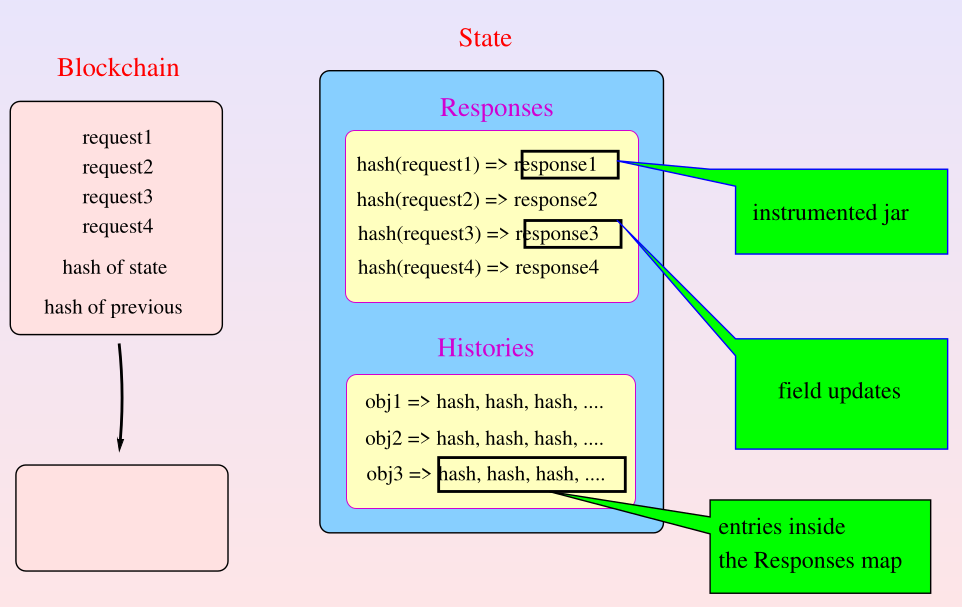
\includegraphics[width=0.8\textwidth]{capitolo3/studio-preliminare/hotmoka-state.png}
  \caption{Lo stato di un blocco nella \textit{blockchain} Hotmoka}
\end{figure}

Lo stato \textit{responses} ha il compito di memorizzare la risposta di ogni transazione che è stata effettuata. Infatti associa l'hash della transazione effettuata ad una determinata risposta. 
La risposta può essere di due tipi:
\begin{itemize}
  \item \textbf{JAR}: se la richiesta a cui è associata corrisponde ad una memorizzazione di un JAR. In questo caso dentro la risposta verrà memorizzato il JAR che è stato inserito in un nodo;
  \item \textbf{Field updates}: se la richiesta a cui è associata corrisponde alla creazione di un oggetto oppure all'invocazione di metodi che modificanoo lo stato. In questo caso la risposta conterrà o l'oggetto istanziato, oppure il valore dei campi che sono stati aggiornati dall'invocazione di un metodo.
\end{itemize}

L'implementazione tipica di questo stato viene data attraverso l'utilizzo di un \textit{Merkle} tree, la quale \textit{Merkle root} viene memorizzata dentro il blocco che deve essere salvato in \textit{blockchain}

Lo stato \textit{histories} invece viene utilizzato per associare ad ogni oggetto, l'hash delle richieste che per ultime hanno modificato un campo dell'oggetto in modo tale da poter ricostruire il suo stato. Da questo ne consegue che se un oggetto ha 3 campi, la sua storia potrà essere lunga al massimo tre, visto che si terrà sempre l'ultima richiesta che ha modificato un campo.

%%%%%%%%%%%%%%%%%%%%%%%%%%%%%%%%%%%%%%%%%%%%%%%%%%%%%%%%%%%%%%%%%%%%%%%%%%%%%%%%%%%

\subsection{Lo standard ERC721}
Per \textit{ERC} (\textit{Ethereum Request Comments}) si intendono le richieste di standardizzazione che avvengono nella \textit{blockchain} Ethereum per la scrittura di \textit{smart contract}. Sono associate ad un numero progressivo e quella che gestisce gli NFT è stata la numero 721. Lo standard ERC721 viene impiegato per lo sviluppo di \textit{smart contract} per la gestione di NFT. \\

\begin{figure}[h!]
  \centering
  
\includegraphics[width=0.3\textwidth]{capitolo3/open-zeppelin-logo.png}
  \caption{Logo dell'azienda OpenZeppelin}
\end{figure}

Per lo sviluppo dello \textit{smart contract} in Solidity, è stata utilizzata l'implementazione dello standard \textit{ERC721} più utilizzata e conosciuta nel mondo Ethereum, ovvero quella data dall'azienda OpenZeppelin. Oltre alla sua grande fama e al fatto che è utilizzata dalla maggior parte della \textit{community}, è stata scelta perché non ci sono vulnerabilità attualmente conosciute. \\

Per quanto riguarda invece Hotmoka, essendo una \textit{blockchain} giovane, non è stato implementato alcuno standard per la scrittura di \textit{smart contract} per la gestione di NFT. Per questo motivo, in accordo con il mio \textit{tutor} aziendale, Fabio Pallaro, è stato deciso che avrei provato a scrivere una mia possibile implementazione dello standard ERC721.

%%%%%%%%%%%%%%%%%%%%%%%%%%%%%%%%%%%%%%%%%%%%%%%%%%%%%%%%%%%%%%%%%%%%%%%%%%%%%%%%%%%

\subsection{Il protocollo IPFS (InterPlanetary File System)}
Il protocollo IPFS (\textit{InterPlanetary File System}) è un'alternativa al protocollo internet HTTP che si pone l'obiettivo di creare una rete informatica di portata globale che consenta l'archiviazione delle informazioni in maniera completamente decentralizzata e con elevata scalabilità.

\begin{figure}[h!]
  \centering
  
\includegraphics[width=0.2\textwidth]{capitolo3/ipfs-logo.png}
  \caption{Logo di IPFS}
  \textbf{Fonte}: \href{https://ipfs.io}{https://ipfs.io}
\end{figure}

È attualmente la risposta tecnologica che oggi sembra più concreta ai limiti di HTTP. Il protocollo infatti promette di sostituire HTTP, adottando come base tecnica e concettuale un modello di Decentralizzazione dei contenuti.

Il web di oggi è inefficiente e costoso, dove HTTP permette di scaricare \textit{file} da un computer alla volta invece di ottenere parti degli stessi da più computer contemporaneamente. In più fa riferimento ai file attraverso la \textit{location addressing}, cioè attraverso il nome con il quale vengono riconosciuti in rete. Questo può comportare vari problemi nell'ambito degli NFT. Infatti, se un \textit{hacker} o una qualsiasi altra persona cambiasse un'opera a cui è associato un NFT con un'altra, ma mantenendo lo stesso nome, il sistema non si accorgerebbe di nulla e si perderebbe così l'opera vera e propria, causando un'incongruenza nei dati. 
Uno dei punti di forza di IPFS è proprio il non utilizzare la \textit{location addressing}, ma bensì la \textit{content addressing}. Tramite questo metodo di indirizzamento, ogni file viene associato ad una codice univoco, chiamato CID (\textit{Content ID}), che si basa sul contenuto del file. In questo modo ogni file potrà essere riferito attraverso il proprio CID e non potrà essere sostituito in alcun modo da altri, visto che avranno un CID diverso.

Oltre a questo motivo, è stato scelto di utilizzare IPFS anche per la sua natura decentralizzata che assicura sempre la reperibilità delle opere richieste. Ogni nodo memorizza la rete attraverso una struttura dati chiamata \textit{Merkle DAG (Directed Acyclic Graph)}, dove ogni nodo ha un identificativo ottenuto dall'operazione di \textit{hashing} dei contenuti di esso, ovvero i \text{file} contenuti, attraverso una funzione crittografica come può essere SHA256.

Per quanto concerne il funzionamento e la comunicazione tra i vari nodi della rete, viene utilizzato il protocollo \textbf{\textit{BitSwap}}, ovvero un protocollo per lo scambio di blocchi di dati simile a \textit{BitTorrent}.
Questo protocollo dirige e gestisce la richiesta e l'invio di blocchi da e verso altri \textit{peer} nella rete. \textit{BitSwap} ha due compiti principali: 
\begin{itemize}
  \item acquisire i blocchi richiesti dal client dalla rete;
  \item inviare i blocchi in suo possesso ad altri peer che lo desiderano.
\end{itemize}

IPFS suddivide i \textit{file} in blocchi di dati, identificando ognuno di essi attraverso un CID. Quando qualcuno esegue la richiesta di un \textit{file}, comunica con un nodo della rete il quale, se ha salvato il proprio file glielo invia, altrimenti inizia l'operazione di \textit{discovery}. Qui entra in gioco il protocollo \textit{BitSwap}, il quale prima di tutto invia una richiesta a tutti i \textit{peer} con il quale è connesso dove chiede chi ha il CID di un blocco o direttamente di tutto il \textit{file}. I \textit{peer} vicini gli risponderanno di si se ce l'hanno e no chi non ce l'ha. Questi ultimi comunicheranno con quelli vicini e faranno la stessa domanda, fino a quando la richiesta non passa per un certo numero di \textit{peer} e non viene più inviata. Invece al primo \textit{peer} che ha risposto che ha quel CID, viene fatta la richiesta di inviarglielo. Dopo averlo ricevuto, invia una richiesta di cancellazione della richiesta, in modo tale da non dover far propagare la richiesta del blocco nella rete.

\clearpage

\begin{figure}[h!]
  \centering
  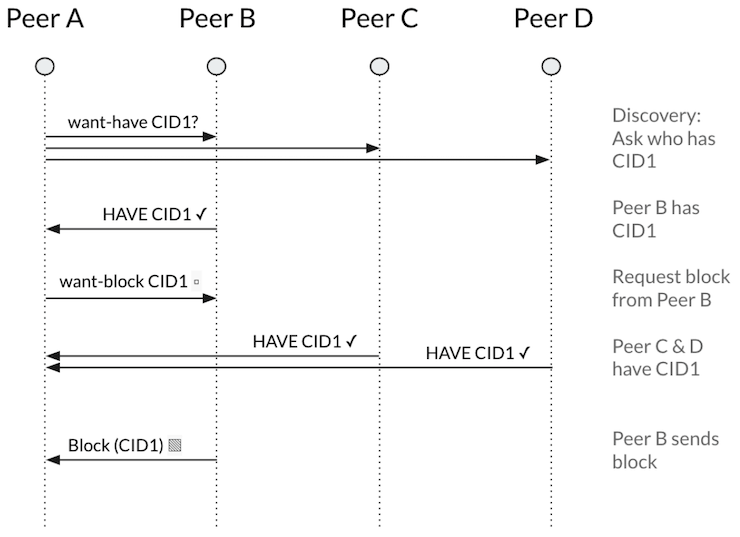
\includegraphics[width=0.8\textwidth]{capitolo3/ipfs-bitswap.png}
  \caption{Esempio di esecuzione del protocllo \textit{BitSwap}}
  \textbf{Fonte}: \href{https://docs.ipfs.io/concepts/bitswap}{https://docs.ipfs.io/concepts/bitswap}
\end{figure}

Essendo IPFS un protocollo a se stante rispetto a HTTP, per poterlo utilizzare in NFTLab avevamo due scelte:
\begin{enumerate}
  \item utilizzare un nodo IPFS locale per connettersi alla rete IPFS;
  \item utilizzare un servizio online per la comunicazione con la rete IPFS.
\end{enumerate}

La prima proposta è stata scartata subito perché solamente complicato ancora di più il sistema che dovevo tenere in piedi per lo sviluppo. Per questo è stata intrapresa la seconda scelta e, in seguito ad una ricerca di quale fosse il servizio più conveniente, è stato scelto Pinata. \textbf{Pinata} offre delle \gls{api} per caricare e prelevare \textit{file} dalla rete IPFS.

\clearpage 
\begin{figure}[h!]
  \centering
  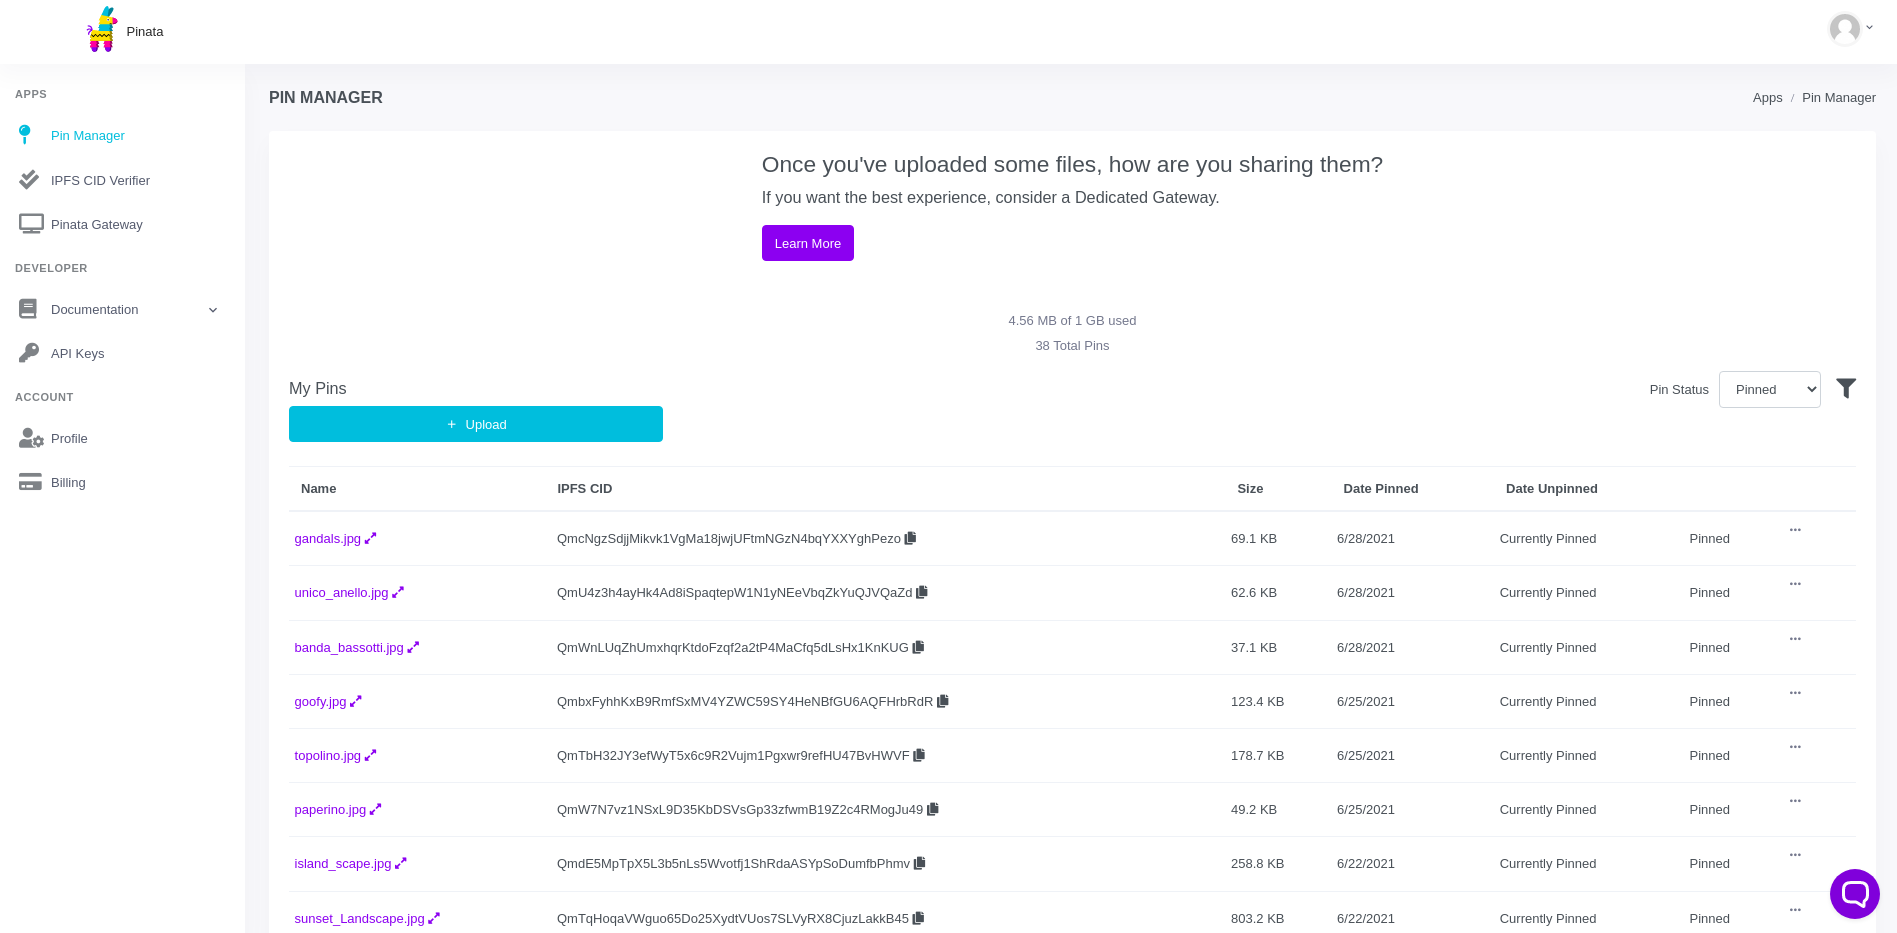
\includegraphics[width=\textwidth]{capitolo3/ipfs-pinata-dashboard.png}
  \caption{\textit{Dashboard} personale di Pinata}
\end{figure}
